\documentclass[bimj,fleqn]{w-art}
\usepackage{times}
\usepackage{w-thm}
\usepackage[authoryear]{natbib}
\usepackage{algorithm}
\usepackage{amsfonts}
\usepackage[hidelinks]{hyperref}
\setlength{\bibsep}{2pt}
\setlength{\bibhang}{2em}

\newcommand{\Y}{{\mbox{\boldmath $Y$}}}
\newcommand{\X}{{\mbox{\boldmath $X$}}}
\newcommand{\Q}{{\mbox{\boldmath $Q$}}}
\newcommand{\bP}{{\mbox{\boldmath $P$}}}
\newcommand{\mbf}[1]{\mbox{\boldmath${#1}$}}

\theoremstyle{plain}
\newtheorem{criterion}{Criterion}
\theoremstyle{definition}
\newtheorem{condition}[theorem]{Condition}
\usepackage[]{graphicx}
\chardef\bslash=`\\ % p. 424, TeXbook
\newcommand{\ntt}{\normalfont\ttfamily}
\newcommand{\cn}[1]{{\protect\ntt\bslash#1}}
\newcommand{\pkg}[1]{{\protect\ntt#1}}
\let\fn\pkg
\let\env\pkg
\let\opt\pkg
\hfuzz1pc % Don't bother to report overfull boxes if overage is < 1pc
\newcommand{\envert}[1]{\left\lvert#1\right\rvert}
\let\abs=\envert

\begin{document}
%\DOIsuffix{bimj.DOIsuffix}
\DOIsuffix{}
\Volume{}
\Issue{}
\Year{2023}
\pagespan{1}{}
\keywords{False discovery rate; Heterogeneous data; Neuroimaging data; Voxel-based lesion-symptom mapping; Weighted p-values}  %%% semicolon and fullpoint added here for keyword style

\title[Weighted FDR Control for VLSM]{False Discovery Rate Control for Lesion-Symptom Mapping with Heterogeneous data via Weighted P-values}

\author[Zheng {\it{et al.}}]{Siyu Zheng\inst{1}} 
\address[\inst{1}]{Department of Epidemiology and Biostatistics, University of South Carolina, SC, United States}

\author[]{Alexander C. McLain\footnote{Corresponding author: {\sf{e-mail: alex.mclain@sc.edu \\ None of the authors have a conflict of interest to report.}}}\inst{,1}}

\author[]{Joshua Habiger\inst{2}}

\author[]{Christopher Rorden\inst{3}}

\author[]{Julius Fridriksson\inst{4}}

\address[\inst{2}]{Department of Statistics, Oklahoma State University, OK, United States}

\address[\inst{3}]{Department of Psychology, University of South Carolina, SC, United States}

\address[\inst{4}]{Department of Communication Sciences and Disorders, University of South Carolina, SC, United States}

%%%%    \dedicatory{This is a dedicatory.}
\Receiveddate{null} \Reviseddate{null} \Accepteddate{null}

\begin{abstract}
Lesion-symptom mapping studies provide insight into what areas of the brain are involved in different aspects of cognition. This is commonly done via behavioral testing in patients with a naturally occurring brain injury or lesions (e.g., strokes or brain tumors). This results in high-dimensional observational data where lesion status (present/absent) is non-uniformly distributed with some voxels having lesions in very few (or no) subjects. In this situation, mass univariate hypothesis tests have severe power heterogeneity where many tests are known \textit{a priori} to have little to no power. Recent advancements in multiple testing methodologies allow researchers to weigh hypotheses according to side-information (e.g., information on power heterogeneity). In this paper, we propose the use of p-value weighting for voxel-based lesion-symptom mapping (VLSM) studies. The weights are created using the distribution of lesion status and spatial information to estimate different non-null prior probabilities for each hypothesis test through some common approaches. We provide a \emph{monotone minimum weight} criterion which requires minimum \emph{a priori} power information. Our methods are demonstrated on dependent simulated data and an aphasia study investigating which regions of the brain are associated with the severity of language impairment among stroke survivors. The results demonstrate that the proposed methods have robust error control and can increase power. Further, we showcase how weights can be used to identify regions that are inconclusive due to lack of power.
\end{abstract}
%% maketitle must follow the abstract.
\maketitle                   % Produces the title.

%% If there is not enough space inside the running head
%% for all authors including the title you may provide
%% the leftmark in one of the following three forms:

%% \renewcommand{\leftmark}
%% {First Author: A Short Title}

%% \renewcommand{\leftmark}
%% {First Author and Second Author: A Short Title}

%% \renewcommand{\leftmark}
%% {First Author et al.: A Short Title}

%% \tableofcontents  % Produces the table of contents.

\section{Introduction}
\label{sec1}

Data arising from neuroscience studies  have considerable statistical issues including a large number of parameters, an unknown spatial dependence structure, and (commonly) low statistical power. Neuroimaging consists of using magnetic resonance imaging (MRI), positron emission tomography (PET), electroencephalography (EEG), or other imaging modalities, to measure various aspects of brain structure and activity.  Data modalities from MRI include functional MRI (fMRI), structural T1 weighted images (T1), and diffusion-weighted imaging (DWI) among others.  These data are typically measured on a voxel level in three-dimensional space.  As imaging technologies improve the number of data voxels per scan has increased, possibly reaching into the millions depending on the spatial resolution of the image. Separate statistical tests are often computed for each location. Therefore, as spatial resolution increases, the opportunity for making erroneous discoveries increases.  This requires some principled thresholding to control for global type I error rate at a level $\alpha$.  Common criteria on the global type I error rate include the familywise error rate (FWER) \citep{Tuk94,NicHol02} and the false discovery rate (FDR) \citep{Benjamini1995}.  

Recent statistical methodology has considered using prior information about the hypotheses to improve results through p-value weighting \citep{Gen06, Roeder2009, Pena2011, Habiger2017, Ignatiadis2021, Lihua2018, Xianyang20}, grouping similar hypotheses \citep{Cai2009, Hu2010,Ignatiadis2016}, or weighting global type I error rate criteria \citep{BenHoc97,BenCoh17,Basetal18}. P-value weighting is a procedure that uses prior information on hypotheses heterogeneity to improve the overall power.  This prior information  -- commonly referred to as \textit{side-information} -- can consist of results from previous studies on the most `promising' hypotheses \citep{LiBar17,LiBar19,Lihua2018}, covariate data indirectly related to the hypotheses \citep{Ignatiadis2021}, or information related to the heterogeneity in the power functions of the hypotheses \citep{Pena2011,Habiger2017}.  The goal of a p-value weighting procedure is to design the weights to maximize the expected number of discoveries while controlling the FWER or FDR.  

  
Modern weighting methods commonly use regression-type approaches to incorporate the side-information into the multiple testing procedure. Commonly these methods use the conditional two-group model where the side-information impacts the probability a test is null and the non-null p-value distribution. For example, \cite{Lihua2018} proposed adaptive p-value thresholding (AdaPT) which adaptively estimates a Bayes optimal p-value rejection threshold. This is done through the use of the Expectation Maximization (EM) algorithm using a set of partially masked p-values. A similar approach referred to as covariate adaptive multiple testing (CAMT) by \cite{Xianyang20}, also uses the EM algorithm with their M step being expressed in terms of the ratio of alternative and null distributions which is modeled using the beta density. \cite{Ignatiadis2021} proposed Independent Hypothesis Weighting (IHW) which divides all tests into several independent folds. For each fold, the estimated weight function can be learned from the p-values and covariates in the remaining folds. Similar to the AdaPT, IHW estimates the null probability and non-null distribution based on a conditional two-group model via an EM algorithm. AdaPT and IHW have been shown to provide finite sample FDR control, while CAMT can provide asymptotic FDR control. \cite{Cai2021} proposed a locally adaptive weighting and screening (LAWS) method to deal with spatial multiple testing problems. The LAWS procedure estimates the weights by using the spatial structure through a kernel screening method and can control the FDR asymptotically. \cite{BocLee18} proposed an FDR control multiple testing method \citep[R package \texttt{swfdr}][]{swfdrpackage} where -- in the spirit of the \cite{Sto02} procedure -- the unknown null indicator is replaced with an indicator the p-value is lower than some threshold. The indicators are used to estimate their associations with the side-information. 


In this paper, we expand the Weighted Adaptive Benjamini Hochberg (WABH) procedure proposed by \cite{Habiger2017} to incorporate heterogeneous non-null probabilities and effect sizes. Further, we demonstrate how our methods are flexible to specific statistical models and are tailored to perform well in low-power settings, which are common in our application to voxel-based lesion-symptom mapping (VLSM) analyses \citep{Batetal03,Roretal07}. Further, WABH is known to be robust to poor estimation of the parameters governing the impact of the side-information on the weights. No previous methods are available that are designed for low-power settings and are robust to misspecification of the weights. In general, this procedure can be applied to any situation where the p-values arise from mass univariate logistic regression. Below, we detail the statistical issues that arise within VLSM and the solutions provided by our testing procedure. 


\subsection{Voxel-based lesion symptom mapping}\label{sec.VLSM}


A main goal of research in neuroscience is to identify and examine areas of the brain related to behavioral or cognitive functions.  A common method is to use subjects with a recent brain injury (e.g., from a traumatic brain injury, epilepsy, or stroke) to map some domain of cognition to specific regions of the brain. This can provide theoretical insights regarding brain function and can also inform clinical treatment. The most popular lesion-symptom mapping approach -- voxel-based lesion-symptom mapping (VLSM) \citep{Batetal03,Roretal07}-- typically relies on structural MRI images (e.g., fMRI, T1, or DWI) where lesion status is measured on  parcellated three-dimensional voxels (e.g. 1 $mm^3$) and relates lesion status to an outcome of interest in each voxel \citep[see][for a recent review of the field]{Karetal17}.  The number of tests in a VLSM can reach millions depending on the resolution of the brain scan.

VLSM analyses are typically mass-univariate tests consisting of computing a simple test statistic (e.g., t-tests, General Linear Models, etc.) for each voxel and then using some multiple testing correction to identify significant associations with regions of the brain. There are a number of statistical issues that complicate such analyses.  First, since studies in humans cannot be designed to injure certain areas of the brain we must rely on naturally occurring injuries \citep{RorKar04}.  This commonly results in lesions being unequally distributed, with some areas/voxels having lesions in a few subjects. For example, stroke-related brain injury is determined by vasculature leading to some regions being far more vulnerable than others. Therefore, the spatial sampling of lesions is not random, and statistical power varies across space. Consider a study of language impairment following left hemisphere injury: we will have low power in regions typically spared in stroke and no power in the right hemisphere (as we have no variability). In response, some have advocated only using voxels that are impacted in, for example, 10\% of subjects to account for this issue \citep{Holetal96}.  Second, it is likely that the areas of the brain that will impact the cognitive outcome will have some spatial clustering. That is, the 3-dimensional coordinates of the voxels will be related to the non-null probability. Ignoring this relationship misses out on an important source of variation in the signal, thereby decreasing the overall power of the procedure. 

The above issues naturally fit into the purview of weighted multiple testing. The naturally occurring injuries in VLSM create heterogeneous power among the voxels. Voxel power is a function of effect size, which is commonly unknown in practice.  In this paper, we propose and provide a straightforward solution consisting of a \emph{monotone minimum weight} criterion, which automatically estimates voxel power and has desirable properties for studies with low to moderate power. Further, we test using plug-in estimates of the non-null probability using state-of-the-art methods (AdaPT and CAMT) which utilize any spatial clustering of signals to gain power. In our data analysis, we demonstrate how the presentation of the impact of weighting is key for transparent reporting of weighted analyses.

The outline of the paper is as follows.  In Section 2, we review multiple testing procedures for data with heterogeneity among the hypotheses.  In Section 3, we discuss how weighted multiple testing procedures can be applied to VLSM in a number of common scenarios. In Section 4, we present results from numerous simulation studies that compare the performance of the proposed method to some common approaches. In Section 5, we present an analysis of $220$ individuals with chronic left hemisphere stroke and identify areas of the brain associated with the severity of aphasia, a language disorder that impacts the expression and comprehension of speech. 



\section{Multiple Testing with Heterogeneous Data}\label{sec.MT_procs}
\subsection{Setup and Notation}
Consider testing null hypothesis $H_m$ based on the random vector $\mathcal{D}_m$ for $m = 1, 2, \ldots, M$. The decision to reject or retain $H_m$ with $\mbf{\mathcal{D}} = (\mathcal{D}_m; m = 1,2,...,M)$ is denoted by $\delta_m(\mbf{\mathcal{D}})\in\{0,1\}$ or $\delta_m$ for short, where $\delta_m$ is 1 if $H_m$ is rejected and is 0 otherwise.  For ease of exposition, we denote the event that a null hypothesis is true (false) by $H_m = 0$ ($H_m = 1$). Table \ref{BHtable} contains our notation for the total number of rejected and retained null hypotheses, incorrectly rejected and retained null hypotheses, correctly rejected and retained null hypotheses, and number of true and false null hypotheses.

The objective of most multiple testing procedures is to define the decision functions $\mathbf{\delta} = (\delta_m; m = 1, 2, ..., M)$ to maximize the expected number of true discoveries/positives $ETP = E[S]$, or minimize some type II error rate, such as the marginal false non-discovery rate $mFNR = {E[U]/E[M-R]}$ \citep{Sun2007}, subject to the constraint that the family-wise error rate $FWER = \Pr(V>0)$ or false discovery rate $FDR = E\left[V/R|R>0\right]\Pr(R>0)$ is not more than a pre-specified level $\alpha$. Variations of the FDR include the positive and marginal FDR, defined as $pFDR = E\left[V/R|R>0\right]$ and $mFDR = E[V]/E[R]$, respectively \citep{Storey2003}. We focus on methods that control the $FDR$ since the WABH procedure, for fixed weights, provides finite $FDR$ control under independence and asymptotic $FDR$ under weak dependence.  However, when deriving optimal weights in what follows, we focus on the $mFDR$ since the expression is more tractable mathematically \citep{CaiSun17} and results in an asymptotically equivalent procedure within our framework.  We note that weak dependence is reasonable in VLSM because p-values are likely to be correlated within regions or clusters of voxels but are nearly independent across distant regions. Simulation studies later explore the effect of dependence in more detail. For situations where the distinction between $mFDR$ and $FDR$ error rates and corresponding procedures is critical, see \cite{heller2021optimal}.

\begin{table}[b]\center
\caption{\label{BHtable} Notation for various hypothesis testings subgroups based on if the null hypothesis is true ($H_m = 0$) or false ($H_m = 1$), and if the tests were rejected ($\delta_m = 1$) or not rejected ($\delta_m = 0$).}
\begin{tabular}{c|cc|c} \hline\hline
& $\delta_m = 0$ & $\delta_m = 1$ & Total \\ \hline
$H_m = 0$ & $T$ & $V$ & $M_0$ \\
$H_m = 1$ & $U$ & $S$ & $M_1$ \\ \hline
&$M - R$ & $R$ & M \\
\end{tabular}
\end{table}

\subsection{Weighted BH Methods}
Many multiple testing procedures have been developed for p-value statistics $\bP = (P_m; m = 1, 2,\ldots, M)$.  The basic idea is to find a p-value threshold $t$ for rejections and define $\delta_m(\bP) = I(P_m \leq t)$ where $I(\cdot)$ is the indicator function.  The well-known \cite{Benjamini1995}, or BH, procedure is implemented by finding the threshold $t_{BH} = \alpha k/M$ where $k = \max\left\{m:P_{(m)}\leq \alpha m/M\right\}$ and $P_{(m)}$ is the $m$th order p-value.  The BH procedure is then given by $\delta_m(\bP) = I(P_m \leq t_{BH})$. \cite{Benjamini1995} showed that if p-values from true null hypotheses are mutually independent and independent of p-values from false null hypotheses, then this procedure has $FDR = \pi_0 \alpha \leq \alpha$, where $\pi_0 = M_0/M$ is the proportion of true null hypotheses. Adaptive FDR procedures (called ABH henceforth), leverage the fact that the BH procedure has FDR $=\pi_0\alpha$ by estimating $\pi_0$ via $\hat{\pi}_0$ and apply the BH procedure at level $\alpha/\hat\pi_0$ \citep{Storey2004}. 


Recent work has further improved upon the BH and ABH procedures by incorporating heterogeneity through p-value weighting.  For example, letting $w_1, w_2, ..., w_M$ be weights satisfying $M^{-1}\sum_mw_m = 1$, the weighted BH procedure (WBH) in \cite{Gen06} operates by applying the BH procedure to the weighted p-values denoted by $Q_m = P_m/w_m$. \cite{Roeder2009} showed that the WBH procedure provides FDR control under a finite mixture model for the p-values considered in \cite{Genovese2002}, among others. Optimal weights for the WBH procedure can depend on heterogeneous prior probabilities for the states of the null hypotheses \citep{Roeder2009,Hu2010,LiBar17,Lihua2018,Xianyang20,LiBar19}, heterogeneous power functions \citep{Pena2011} or both \citep{Cai2009,Habiger2017, Ignatiadis2021}.  



\cite{Habiger2017} proposed the WABH procedure by applying the adaptive BH procedure to weighted p-values as follows: (i) compute weighted p-values via $Q_m = P_m/w_m$ with $\Q = (Q_m; m = 1, 2,\ldots, M)$, (ii) estimate $\hat\pi_0 = \{\sum_m I(Q_m\geq \kappa) + 1\}/\{M(1-\kappa)\}$, (iii) compute threshold $t_{WABH} = \min\left\{\alpha, k \alpha/(\hat\pi_0 M)\right\}$ where $k = \max\left\{m: Q_{(m)}\leq m \alpha/(\hat\pi_0 M)\right\}$, and (iv) compute $\delta_m(\Q) = I(Q_m\leq t_{WABH})$. We utilize this procedure since it can incorporate prior information regarding the heterogeneity of the power functions and the prior null probabilities. Other WABH methods, such as \cite{ramdas2019unified} and \cite{biswas2022new}, have not considered heterogeneity of the power functions (though they do consider other useful features not required for our data example). \cite{Habiger2017} showed that for reasonably specified weights the WABH procedure controls the FDR asymptotically and has higher ETP than the WBH and ABH procedures. In particular, as long as the utilized weights are positively correlated with optimal weights the procedure still controls the FDR and is more powerful than unweighted procedures. This allows for a procedure that incorporates heterogeneity across tests in applications where the precise nature and degree of heterogeneity isn't well known, but may be estimated or reasonably specified. The first step in utilizing such a procedure is to specify optimal Oracle weights.



\subsection{Optimal Oracle Weights}\label{sec.opt.weight}
Optimal Oracle weights are allowed to depend on heterogeneous prior probabilities and/or power functions.  Suppose, for example, $P_m$ has null CDF $F_0(t) = \Pr(P_m\leq t|H_m=0)=t$ and alternative CDF $F_m(t) = \Pr(P_m\leq t|H_m=1)$.  Further let $\pi_m = \Pr(H_m = 1)$ be the prior probability that $H_m$ is non-null for $m = 1, 2, ..., M$.   Suppose, for the moment, the Oracle situation where the weighted p-value threshold $t_m$ along with $\pi_m$ and $F_m$ for each $m$ are known.  The weighted p-value decision rule can be written $\delta_m(Q_m) = I(Q_m \leq t) = I(P_m \leq w_mt) \equiv I(P_m \leq t_m)$. 


The calculation of the optimal weights reduces to maximizing the expected number of true positives, $ETP(\mbf{t};\mbf{\pi}) = \sum_m \pi_m F_m(t_m)$ where $\mbf{t}=(t_1,\ldots,t_M)$ subject to the constraint that $M^{-1}\sum_mt_m = t$. That is, the objective is to find
%
$$\max_{\mbf{t}}ETP(\mbf{t};\mbf{\pi}) \mbox{ such that } mFDR(\mbf{t};\mbf{\pi}) = \frac{\sum_m (1-\pi_m)t_m}{\sum_m (1-\pi_m)t_m+\sum_m \pi_m F_m(t_m)} \leq \alpha,$$
%
which can be solved via Lagrange multipliers \citep{Habiger2017}. 

One can calculate the optimal weights for p-values arising for various distributional assumptions. We go through the calculation details for when the $P_m$'s arise independently from a normally distributed test statistic that has mean $g_m$ and unit variance since they align with the assumptions of our models. We discuss our assumptions and calculations of $g_m$ in Section \ref{sec.w.VLSM}. In this situation, the power of a test of size $t$ is $F_m(t) = \bar{\Phi}\left\{\bar{\Phi}^{-1}(t) - g_m\right\}$ where $\bar\Phi(\cdot) = 1- \Phi(\cdot)$, and $\Phi(\cdot)$ is a standard normal distribution function. The expression for $f_m(t) = \frac{d}{dt}F_m(t)$ is 
%
\begin{equation}\label{eq.f}
f_m(t_m) = \frac{\phi\{\bar\Phi^{-1}(t_m) - g_m)\}}{\phi\{\bar\Phi^{-1}(t_m)\}},
\end{equation}
%
where $\phi(t)$ is the standard normal density function and
%
$$\frac{d}{dt_m}\left\{mFDR(\mbf{t};\mbf{\pi}) - \alpha\right\} = mFDR'(t_m,\pi_m,\alpha) = (1-\alpha)(1-\pi_m)-\alpha \pi_mf_m(t_m),$$ 
% 
Setting $\pi_mf_m(t_m) - \lambda mFDR'(t_m,\pi_m,\alpha)=0$ yields the following expression
%
$$f_m(t_m)=\frac{\lambda(1-\pi_m)(1-\alpha)}{\pi_m(1+\lambda\alpha)} = c_\alpha(\lambda;\pi_m), $$
%
where the solution in terms of $t_m$ is
\begin{equation} \label{eq.t}
 t_m(\lambda) = \bar\Phi\left[0.5g_m + \log\{c_\alpha(\lambda;\pi_m)\}g_m^{-1}\right].
\end{equation}
The Lagrange multiplier is found by solving
\begin{equation}\label{eq.lambd}
\sum_m (1-\pi_m) t_m(\lambda) - \alpha\left[\sum_m (1-\pi_m) t_m(\lambda) + \sum_m \pi_m F_m\{t_m(\lambda)\}\right] = 0
\end{equation}
for $\lambda$.  The weights are then given by $w_m = t_m(\hat \lambda)\{M^{-1}\sum_m t_m(\hat \lambda)\}^{-1}$ where $\hat{\lambda}$ is the solution to (\ref{eq.lambd}). Once the weights are calculated the WABH procedure can be implemented.


The above Oracle procedure requires that the marginal distributions $\pi_m F_0(t) + (1-\pi_m)F_m(t)$ be correct, and $\{(\pi_m,F_m)_{m=1,\ldots,M}\}$ be fixed for mFDR control. That is, mFDR control would be provided for any joint distribution that results in these marginal distributions.  For a related concept see Proposition 2.2 in \cite{heller2021optimal}.  




\section{Estimation of weights in VLSM}\label{sec.w.VLSM}
VLSM is a procedure that measures the strength of the association between lesion status and a cognitive outcome, independently for each voxel \citep{Batetal03}.  Let $X_{im}$ denote a measure of whether brain voxel $m$ has a lesion for person $i$, $m=1,2,\ldots,M$ and $i=1,2,\ldots,n$. Let $Y_i$ denote the cognitive measure of interest for person $i$, which we assume to be continuous. Further, let $X^+_{im} = h(\sum_{j \neq m} X_{ij})$ be a measure of the total lesion size excluding voxel $m$ for person $i$ for some function $h$.  Below we consider $X^+_{im} \in \mathbb{R}$, but incorporating multidimensional $X^+_{im}$ is straightforward. Since voxel damage can only be a detriment to the cognitive outcome we consider $H_m$ to be one-sided hypothesis tests, however, the methods are easily generalized to two-sided tests.  We focus on logistic regression since the spatial dependence within the $X$'s can be generated by factors that are independent of the association of interest, and the total lesion size ($X^+_{im}$) can be adjusted for as a nuisance confounder \citep{Karetal04,Arnetal18,Roretal07}.

The optimal oracle weights in Section \ref{sec.opt.weight} require the specification of $g_m$ and $\pi_m$ in equations (\ref{eq.f}) and (\ref{eq.lambd}). To estimate the $\pi_m$'s we use existing general methods (discussed in Section \ref{sec.prior.prob}). In Section \ref{sec.pow.est}, the heterogeneous $g_m$'s are calculated by utilizing heterogeneous standard error calculations and prior knowledge that the power of the tests is low. Our resulting WABH algorithm is outlined in Section \ref{sec.eff.size}. 



\subsection{Estimation of prior null probabilities using known methods}\label{sec.prior.prob}

Ideally, values for the prior null probabilities ($\pi_m$) can be based on previous studies and expert knowledge.  When this is not possible, there are various approaches to estimating $\pi_m$. Here, we focus on the AdaPT and CAMT procedures \citep{Lihua2018,Xianyang20} due to the ease of implementing them in statistical software. AdaPT and CAMT are innovated multiple testing procedures that yield estimates $\pi_m$ and/or $f_m$ conditional on so-called `side-information', denoted by $\mbf{z}_m$. The side-information are pre-specified data about test $m$ hypothesized to be related to $\pi_m$ and/or $f_m$ (examples given below). We utilize these procedures to provide plug-in estimates of $\pi_m$ that we can use to implement the WABH algorithm. We do not use their multiple testing results, or estimates of $f_m|z_m$ (our specification of $f_m|z_m$ is discussed in the following section).



The estimators provided by the the AdaPT and CAMT software are based on the two-groups model, with $P_m|\mbf{z}_m,H_m \sim (1-H_m)f_0 + H_mf_m$ where $f_0$ is the density of $P_m$ under the null, $f_m$ is the conditional density of $P_m$ given $(H_m=1,z_m)$, and $\pi_m = \Pr(H_m=1|\mbf{z}_m)$. To implement estimators, we need to specify a parametric form for the relationship between (i) $\mbf{z}_m$ and $\pi_m$, and (ii) $\mbf{z}_m$ and $f_m$. For example, in our simulation study, $\mbf{z}_m = (\mbf{z}^\pi_{m},\mbf{z}^f_{m})$ consists of the $2\times 2$ coordinates of test $m$ ($\mbf{z}^\pi_{m}$), and the predicted standard error of the regression coefficient ($ \mbf{z}^f_{m}$). For (i), $\log\{\pi_m/(1-\pi_m)\}$ is modeled with natural cubic splines on $\mbf{z}^\pi_{m}$. For AdaPT we assume $f_m$ is a beta density, and for CAMT we assume the ratio $f_m/f_0$ is a beta density. Specifically, a beta$(k_m,1)$ where for (ii), $\log(k_m)$ is modeled with natural cubic splines on $\mbf{z}^f_{m}$. See Section \ref{sec.sim} for more details and Section \ref{sec.data.anal} for the specification of these relationships in our real data analysis.  

AdaPT uses a sophisticated masking an unmasking of p-values to estimate all model parameters (i.e., parameters governing the relationships between $z_m$, and $\pi_m$ and $f_m$) with finite sample guarantees of FDR control. Our implementation of both estimation procedures uses the EM algorithm. We use the estimated $\pi_m$'s in the final iteration of the \texttt{adapt-MT} and \texttt{CAMT} \texttt{R} functions \citep[see][and the package documentations for further details on their estimation procedures]{Lihua2018,Xianyang20}. 

%, 

\subsection{Estimation of effect sizes and MMW criterion}\label{sec.pow.est}

In this section, we develop expressions for estimating $g_m$, which will be used to estimate optimal weights in subsequent sections.  We consider a strictly continuous outcome $Y_i \in \mathbb{R}$ and a binary $X_{im}\in (0,1)$ lesion indicator, which is modeled as a function of $Y_i$ and $X_{im}^+$ with a logistic regression model.  

Let $\mbf{Y}=\{Y_{1},Y_{2},\ldots,Y_{n}\},$ $\mbf{X}_m^+=\{X^+_{1m}, X^+_{2m}, \ldots, X^+_{nm}\}$ and $\mbf{X}_m=\{X_{1m},X_{2m},\ldots,X_{nm}\}$ for $m=1,\ldots,M$.   We consider null hypotheses $H_m:\beta_{1m}=0$ and alternative $H_m:\beta_{1m}>0$ where
%
$$\mbox{logit}\{\Pr(X_{im}=1|Y_i,X_{im}^+)\} = \beta_{0m} + \beta_{1m}Y_i + \beta_{2m} X^+_{im},$$
%
where $\mbox{logit}(p)=\log\{p/(1-p)\}$.  The Wald test p-values are $P_{m} = \bar\Phi(\hat \beta_{1m}/\widehat{SE}_m)$, where $\widehat{SE}_m$ is the estimated standard error of $\hat\beta_{1m}$. The power of a test will depend upon $\beta_{1m}$ and $SE_m$.  Using previous results \cite{VaeSko04}, the standard error of $\hat\beta_{1m}$  can be approximated via
%
\begin{equation}\label{eq.logreg.SE}
SE_m = \left[\frac{(1-R^2_{m})}{n s^2_Y\bar X_m(1-\bar X_m)} \right]^{1/2} + o_p(n^{-1/2})
\end{equation}
%
where $R^2_{m}$ is the coefficient of determination for regressing $\Y$ on $\X_m^+$, $\bar{X_m}=\sum_i(X_{im})/n$, $s_Y^2=\sum_i(Y_{i}-\bar Y)^2/(n-1)$. Then,
%
\begin{equation}\label{eq.logreg.T}
\frac{\beta_{1m}}{SE_m} = \frac{\eta_{m}}{S_{m}} +o_p(n^{-1/2})
\end{equation}
%
where $\eta_{m} = \beta_{1m}s_Y$  and $S_{m}=[(1-R^2_{m})/\{n\bar X_m(1-\bar X_m)\}]^{1/2}$.  Assuming normality of the test statistics, given $g_m = \eta_{m}/{S}_{m}$ the power of a test of size $t$ is $F_m(t) = \bar{\Phi}\left\{\bar{\Phi}^{-1}(t) - g_m\right\}$.  Since $S_m$ can be estimated \textit{a priori}, the heterogeneity in the power can be calculated given the effect size $\eta_m$. To specify $\eta_m$, we assume prior data differentiating $\eta_m$ are unavailable and set $\eta_m=\eta$ for all $m$.  



Figure \ref{Fig.eta.pl} displays an example of the relationship between the weights ($w_m$) and $S_m$ for different $\eta$. This figure also shows the 10\% rule (which is common in practice), where the weights are given by $w_m = MI(\bar X_m \in [0.1,0.9])/(\sum_{k=1}^M I(\bar X_k \in [0.1,0.9]))$. Note that the 10\% rule up-weights tests (i.e., $w_m \geq 1$) with high power (lower $S_m$) and down-weights tests with low power.  \cite{Habiger2017} showed that in low-power settings, optimal weighting schemes have larger weights for tests with higher power and lower weights for tests with lower power. Thus, the intuition behind the 10\% rule is correct, however, a more sophisticated weighting scheme from the optimal weights in Section \ref{sec.opt.weight} is available. 

Since our motivating example is a low-power setting, we define a monotone minimum weights (MMW) criterion for selecting the tuning parameter $\eta$.  In summary, the MMW weights are the specific optimal weights that satisfy the desired monotonicity property while ensuring that weights are not too aggressive. This ensures that tests with higher power have higher weights while minimizing the impact of weighting -- aggressive weighting schemes may result in very large weights for only a few tests while vast majority of tests are essentially ignored due to severe down-weighting.  The MMW arises by choosing $\eta$ as large as possible so that weights are still monotone. The resulting weights are depicted in Figure \ref{Fig.eta.pl} by the solid black line. Note that in Figure \ref{Fig.eta.pl} the MMW weights amount to choosing $\eta = .178$. Choosing $\eta = 0.25$ (dashed line) results in weights that are not monotone while for $\eta = 0.1$ (dotted line) the weights are monotone but more aggressive than the MMW weights. Consequently, $\eta = 0.1$ results in a few large weights and most weights being $\approx 0$. 



\begin{figure}[t]
\centering
\includegraphics[scale=0.4]{Figures/Weight_plot_logit_w_MPS.pdf}
\caption{\label{Fig.eta.pl} Estimated p-value weights ($w_m$) by their predicted standard error ($S_m$) for the aphasia data where $\eta = 0.1$ (black dotted), $0.178$ (black solid), and $0.25$ (black dashed), along with the 10\% rule (gray solid).}
\end{figure} 

The weights also vary as a function of $\pi_m$, but are monotone in $\pi_m$ by definition. As a result, the MMW criteria is set for monotonicity in $S_m$ for a fixed value of $\pi_m = \tau$. The role of $\tau$ is discussed below. The general expression for MMW weights is provided in Theorem \ref{thm.1} below as a function of Lagrange multiplier $\lambda$, which is set such that equation (\ref{eq.lambd}) holds. 



\begin{theorem}\label{thm.1}
For any $\lambda$ and $\tau\in [0,1]$ such that $\log\{c_\tau(\lambda)\}>0$ where $c_\tau(\lambda) \equiv  \lambda(1-\tau)(1-\alpha)/\{\tau(1+\lambda \alpha)\}$, the maximum $\eta$ such that $w_{m} - w_{m^\prime}\geq 0$ for all $S_{m} - S_{m^\prime}\leq 0$ and $\pi_m=\pi_{m'} = \tau$, is given by $\tilde{\eta} = S_{(1)}\sqrt{2\log\{c_\tau(\lambda)\}}$ where $S_{(1)} = \min_m(S_m)$. In this case, the thresholds are given by
%
\begin{equation} \label{eq.t_eta}
 \tilde t_{m}(\lambda) = \bar\Phi\left\{0.5\left(\frac{\tilde{\eta}}{S_{m}}\right) + \log\{c_\tau(\lambda)\}\left(\frac{\tilde{\eta}}{S_{m}}\right)^{-1}\right\}.
\end{equation}
%
\end{theorem}


\noindent A proof of this theorem is given in Section A of the Supporting Material. 

Under the MMW criteria, the impact of weighting is minimized in that proportion of up-weighted tests is maximized among all $\eta$ values with non-increasing weights for $S_m \geq S_{(1)}$ and $\pi_m = \tau$. The value of $\tau$ guarantees that the weights satisfy the MMW criteria for all $m$ with $\pi_m=\tau$. When one uses $\pi_m=\hat\pi$ for all $m$, set $\tau=\hat \pi$ to have MMWs for all $m$. The main utility of $\tau$ is for cases when $\pi$ is computed as in Section \ref{sec.prior.prob}, where there is a range of $\pi_m$ values. For this situation, the MMW criteria holds for all tests with prior non-null probabilities equal to $\tau$. To clarify the behavior of the weights for $\pi \neq \tau$, consider the following proposition (proof in the supplemental materials).

\textit{\textbf{Proposition 3.2} If the weights satisfy the MMW criteria at $\tau$, then for all $\pi_m=\pi_{m'} < \tau$, if $S_{m} - S_{m^\prime}\leq 0$ then $w_{m} - w_{m^\prime}\geq 0$. }

As a result, if one uses MMW at $\tau$, then the weights will be monotone in $S$ for any $\pi<\tau$, while for $\pi>\tau$ the weights will be non-monotone for some $S\geq S_{(1)}$ (a result of Theorem \ref{thm.1}). Additionally, if $\tau = \max(\mbf{\pi})$ then the weights will be monotone for each $\pi$ in the data. Setting $\tau = \max(\mbf{\pi})$ is effective for studies that are low in power since all weights will be monotone in $S$ (for a fixed $\pi$). For studies with more robust power, we find setting $\tau$ to mean or $q$th percentile of the observed $\pi_m$'s can give better results since tests with large $\pi$ and small $S$ do not need to have a large weight. In this situation, weights for tests with $\pi_m>\tau$ are non-monotone (e.g., see the dashed line in Figure \ref{Fig.eta.pl}). 

%If $\log\{c(\lambda)\}>0$ does not hold there does not exists an $\eta$ where the optimal weights are monotone decreasing in $S_m$ at $\pi_m=\tau$ for all $m$. In this situation, $\tau$ can be changed or $\eta$ can be set manually. 

\subsection{WABH algorithm}\label{sec.eff.size}

A general form for implementing the WABH procedure at level $\alpha$ is given in Algorithm \ref{wabh.algorithm1}. \texttt{R} code to run our proposed testing procedure along with data to replicate the results of our analysis in Section \ref{sec.data.anal} are available on GitHub \citep{McLZhe22}. Our implementation uses logistic regression to obtain $S_m$ and $P_m$ in step 1. The functional form between $\mbf{z}_m$ and $\pi_m$, and $\mbf{z}_m$ and $f_m$ is required for step 3. While our procedure only uses the estimates of $\pi_m$ in step 3, specifying a plausible model for $f_m|\mbf{z}_m$ is important since a poor model can have a negative impact on the estimates of $\pi_m$.  We estimate $\pi_0$ using the average estimated $1-\pi_m$; using other methods \citep[e.g.][]{Sto02} could increase the robustness of the procedure by decreasing the dependency of the algorithm on the estimated $\pi_m$'s. 


\begin{algorithm}[t]
\caption{A general form for the WABH algorithm using AdaPT or CAMT.} \label{wabh.algorithm1}
\begin{enumerate}
    \item Initialize: specify the functional form between the side-information ($\mbf{z}_m$), $\pi_m$, and $f_m$.
    \item For $m=1,2,\ldots,M$ 
    \begin{enumerate}
        \item Compute $\bar X_m$ and $R^2_m$ to obtain $S_m$ in equation (\ref{eq.logreg.T}).
        \item Compute the unweighted p-value $P_m$.
    \end{enumerate}
    \item Implement AdaPT or CAMT on $P_m$, extract estimates of $\pi_m$ for all $m$.
    \item Specify $\eta_m=\eta$ directly or specify $\tau$ and compute $\tilde\eta = S_{(1)}\sqrt{2\log\{c_\tau(\lambda)\}}$. 
    \item Compute the optimal weights by 
    \begin{enumerate}
    \item plugging $(g_m=\eta_m/S_m,p_m)$ into (\ref{eq.lambd}) and solving for $\hat{\lambda}$, and
    \item compute $w_m = t_m(\hat \lambda)\{M^{-1}\sum_m t_m(\hat \lambda)\}^{-1}$ using $t_m(\hat \lambda)$ in (\ref{eq.t}).
    \end{enumerate}
    \item Compute weighted p-values $Q_m = P_m/w_m$.
    \item Implement adaptive BH procedure:
    \begin{enumerate}
    \item find $k^\ast = \max\left\{m: Q_{(m)}\leq m \alpha/(\hat\pi_0 M)\right\}$ where $\hat\pi_0 = M^{-1}\sum_m (1 - \pi_m)$, and 
    \item compute $\delta_m(\Q) = I(Q_m\leq t_{WABH})$ where $t_{WABH} = \min\left\{\alpha, k^\ast \alpha/(\hat\pi_0 M)\right\}$.
    \end{enumerate}
    
\end{enumerate}

\end{algorithm}


Though the WABH procedure provides some robustness in terms of FDR control when weights are estimated with the test data (especially here where they are roughly consistently estimated), for theoretical guaranteed FDR control weights would need to be estimated using independent data. One option is to use sample splitting, where part of the data (e.g., 20\%) is used to estimate the weights and the remaining data is used to perform hypotheses testing. Simulation studies presented in Section B of the Supplemental Materials suggest that while sample splitting can reliably control the FDR, the loss in power in exchange for this guaranteed control is too significant in the sample sizes that are common in VLSM studies. Another issue with sample splitting for VLSM is that for many voxels less than 5\% of of subjects have damage. In this case, sample splitting results in $X_{im}=0$ for all $i$ for many $m$ -- where weights cannot be estimated. However, if previous data are available to estimate the weights, then the WABH procedure can provide guaranteed FDR control.


There are multiple measures of the impact of weighting such as the proportion of up-weighted tests (i.e., those with $w_m \geq 1$), the maximum weight, and the proportion of tests that are \textit{inconclusive} (e.g., those with $w_m < 0.1$). Inconclusive tests are those that are essentially ignored by the testing procedure, i.e., they are likely to be not rejected due to their low weight. Reporting tests that are inconclusive is an important step in implementing the WABH (or other weighting procedures) so that the hypotheses essentially not included in the testing procedure can be known. 

\section{Simulation Study}\label{sec.sim}


To test the properties of the proposed methods we performed simulation studies with logistic regression models. We considered a two-dimensional $100 \times 100$ grid of data.  Let $\mathcal{S}_1$ index the set of false nulls. The coordinates of the tests in $\mathcal{S}_1$ were simulated from a zero-mean Gaussian random field (GRF) with $\Sigma_{s}(m,m^\prime) = \exp\{-(||\mbf{z}^\pi_{m} - \mbf{z}^\pi_{m'}||_2/s)^2\}$ where $\mbf{z}^\pi_{m}$ is the two-dimensional coordinates for point $m$ and $||\cdot||_2$ is the $l_2$-norm.  The tests in $\mathcal{S}_1$ were those with the largest $K = ||\mathcal{S}_1||$ simulated values. The data were generated via
%
\begin{equation}\label{eq.sim.study}
\mbox{logit}\{\Pr(X_{im}=1|Y_i,b_i)\} = \alpha^\ast_0 + \alpha^\ast_{0m} + \alpha^\ast_{1m}Y_i+ b_i,
\end{equation}
%
where $\alpha^\ast_0 = -1$, $\alpha^\ast_{0m}$ follows a zero-mean GRF with covariance function $C^{2} \Sigma_{50}(m,m^\prime)$, $\alpha^\ast_{1m}\sim U(0,2\theta)$ for all $m \in \mathcal{S}_1$ ($\alpha^\ast_{1m}=0$ otherwise), $b_i \sim N(0,0.8^2)$, and $Y_i = 0.5b_i + \epsilon_i$ where $\epsilon_i \sim N(0,0.5^2)$. Recall from (\ref{eq.logreg.SE}), that the power heterogeneity is driven by $Var(X_{im})=\bar X_m(1-\bar X_m)$, which will be a function of $\alpha^\ast_{0m}$ in that extreme $\alpha^\ast_{0m}$ will have low $Var(X_{im})$.  Thus, $C^{2}=Var(\alpha^\ast_{0m})$ controls the amount of power heterogeneity among the tests. The simulation settings were varied over all cominations of $C\in\{0.5, 1.5,3\}$, $s\in \{0.01, 5, 10\}$, $K\in\{100, 500\}$, and $\theta \in \{0.25,0.5,0.75\}$. Examples of $\mbf{X}$ and $\mathcal{S}_1$ are given in Section D of the Supporting Material. All simulations used $n=200$. 



\begin{figure}[t]
\begin{center}
\includegraphics[width= 6.4in, height=4.2in]{Figures/SimulationPlotFDR5.pdf} 
\end{center}
\vspace{-.2in}
\caption{Average false discovery rates (FDR) by power heterogeneity ($C$), number of true signals ($K$), effect size ($\theta$), and spatial dependence ($s$) for $M=10000$ tests and $n=200$.}\label{fig.bin.sim1}
\end{figure}



The fitted model for the $m$th test was
%
$$\mbox{logit}\{\Pr(X_{im}=1|Y_i,X_{i}^+)\} = \alpha_{0m} + \alpha_{1m}Y_i + \alpha_{2m}X_{im}^+  $$
%
where $X_{im}^+ = \mbox{logit}\{(M-1)^{-1}\sum_{j \neq m} X_{ij}\}$. The p-value weights were estimated using Algorithm \ref{wabh.algorithm1} where $\pi_m$ was estimated using AdaPT, or CAMT. For both procedures, 
%
\begin{equation}\label{eq.pm.model}
\log\{\pi_m/(1-\pi_m)\} = \gamma_0  + \gamma_1 h_5(z_{m1}^\pi) + \gamma_2 h_5(z_{m2}^\pi) + \gamma_3 h_5(z_{m1}^\pi z_{m2}^\pi) 
\end{equation}
%
where $z_{mj}^\pi\in \{1,2,\ldots,100\}$ is coordinate $j$ of test $m$ and $h_5(z)$ is a vector of $5$ degree natural cubic splines with evenly spaced knots evaluated at $z$. Further, $\log(k_m) = h_5(S_m)$. To select $\eta$ we used the MMW criteria with $\tau = 0.5$ or $0.9$. We note that for AdaPT and CAMT the the beta assumption on the distribution of non-null p-values (discussed in Section \ref{sec.prior.prob}) is likely misspecified. We also tested an inverse Gaussian assumption for AdaPT and found largely similar results (not shown). Similar to \cite{Xianyang20}, for CAMT we cap the maximum $\pi_m$ at 0.9 to prevent too large $\pi$ and guard against the dominance of the prior (this is the default in the \texttt{CAMT} package). We also included the Adaptive BH, IHW, LAWS, and SWFDR procedures in the simulation. Adaptive BH was implemented with $\hat\pi_0$ being estimated using \cite{Sto07} with a threshold set at $0.05$ as suggested for dependent data \citep{Blanchard2009}. IHW was fitted with one covariate ($S_m$), as this was all the software allowed, with five-folds and automatic selection of the number of bins. SWFDR was fitted with a design matrix consisting of the two-dimensional coordinates and $S_m$ to estimate the null probability for each test. To fit LAWS we used a threshold of $0.9$ (the default) with a Gaussian kernel and bandwidth set to 4.5. LAWS does not model the non-null p-value distribution via covariates, thus $S_m$ was not used.

The methods are compared in terms of $FDR = B^{-1}\sum_b I(R_b>0)(V_b/R_b)$ and $Power = ETP/K$ ($ETP = B^{-1} \sum_b S_b$) where $S_b$, $V_b$ and $R_b$ denote the number of correct discoveries, false discoveries and total discoveries from the $b$th iteration. Procedures set $FDR$ control level to $\alpha=0.05$. All simulations were run for $B=500$ iterations.  For brevity, we show the WABH when $\pi_m$ was estimated using CAMT with $\tau=0.9$ only. Section D of the Supporting Material contains results of WABH with AdaPT and other $\tau$ values along with other common methods. 


\begin{figure}[t]
\begin{center}
\includegraphics[width= 6.4in, height=4.2in]{Figures/SimulationPlotETP5.pdf} 
\end{center}
\vspace{-.2in}
\caption{Estimated power ($ETP/K$) by the power heterogeneity ($C$), number of true signals ($K$), effect size ($\theta$), and spatial dependence ($s$) for $M=10000$ tests and $n=200$.}\label{fig.bin.sim2}
\end{figure}



In Figure \ref{fig.bin.sim1}, we present summarized FDR results of simulation studies. The AdaPT, Adaptive BH, IHW, and WABH procedures all controlled the FDR with values that are less than or close to the nominal level in all settings. The CAMT had high $FDR$ when the proportion of false null hypotheses or expected effect size ($\theta$) was low. For example, when $K=100$ and $\theta=0.25$, the $FDR$ ranged from $0.2-0.6$ and $0.2-0.3$ in the low to moderate, and high heterogeneity settings, respectively. For $K=100$ and $\theta=0.75$, the CAMT $FDR$ ranged from $0.06-0.16$, while for $K=500$ the FDR was controlled reasonably well for $\theta \geq 0.5$. The LAWS procedure also resulted in $FDR$ values that were above the nominal level when $\theta=0.25$, and some $\theta=0.5$ settings. Lastly, the $FDR$ for the SWFDR procedure was above the nominal level in all high heterogeneity settings. 


In Figure \ref{fig.bin.sim2}, we present summarized power results of simulation studies. Overall, among the procedures that control $FDR$ in most settings (i.e., AdaPT, Adaptive BH, IHW, and WABH) the WABH procedure had the largest power. AdaPT had larger power for $\theta = 0.75$, $K=500$ when $s \leq 5$. For $\theta=0.75$, the LAWS procedure controlled the FDR and had the largest power (CAMT has larger power only when the FDR$\geq \alpha$). Further, LAWS performed well (FDR controlled and high power) for $\theta=0.5$ and $K=500$. As a result, the LAWS procedure appears to perform well in high-powered settings, however, such settings are not likely in our application of interest. 

Section C of the Supplemental Material present results from  simulation studies designed to test the robustness of the proposed method to dependence in the p-values under the null-hypothesis. Briefly, the results of these studies were largely similar to those presented herein. 




\section{Data Analysis}\label{sec.data.anal}


Our sample was drawn from the population described in detail by \cite{Youetal15}, and follows the same inclusion/exclusion criteria, behavioral testing, and behavioral analyses. In brief, all participants were adults with chronic left-hemisphere stroke and aphasia. All individuals were scanned using a 3T MRI scanner. Lesions were obtained by hand by an expert on a high-resolution T2-scan for optimal identification of lesion boundaries. Lesions were coregistered to the individual's T1 scan. Each individual’s lesion was warped to have a common size and shape through enantiomorphic normalization \citep{Nacetal08} using our clinical toolbox \citep{Roretal12}. Therefore, for each individual, the lesion was mapped as a binomial volume with a resolution of $181\times 217 \times 181$ voxels (each 1mm$^3$), though many of these voxels are outside the brain or have zero damage for all subjects. For this study, we included the $220$ individuals enrolled at the time of these analyses. Data from $834582$ \textit{candidate voxels} -- voxels with damage to at least one subject -- were considered. 

To fit WABH we used CAMT to estimate $\pi_m$ with the MMW criteria and $\tau = 0.9$. The side-information consists of $\mbf{z}_m^\pi$ the $3$-dimensional voxel coordinates and $S_m$. The relationship between $\mbf{z}_m^\pi$ and $\pi_m$ was similar to \eqref{eq.pm.model} with natural cubic splines on all three coordinates and all two-way interactions. We used 12 degrees of freedom for the splines, which had the smallest BIC among the many values tested. The comparison methods included the 10\% Rule, BH, ABH, AdaPT, and CAMT methods. For AdaPT, penalized regression splines with an automatic degree of freedom selection were used to relate $\mbf{z}_m^\pi$ and $\pi_m$ and $S_m$ with $f_m$. We attempted an analysis with LAWS on this data also but it was not computationally feasible and failed to converge. Part of the issue is that LAWS requires a full cubic 3D structure that resulted in $2\times 10^6$ tests (more than twice the tests of other procedures). For AdaPT and the WABH with AdaPT, we removed voxels with damage in less than 0.5\% of subjects due to convergence issues. Codes and data to replicate the data analyses are available on GitHub \cite{McLZhe22}.

\begin{figure}[t]
\centering
\begin{tabular}{ccccccc} 
(a) & (b) \\
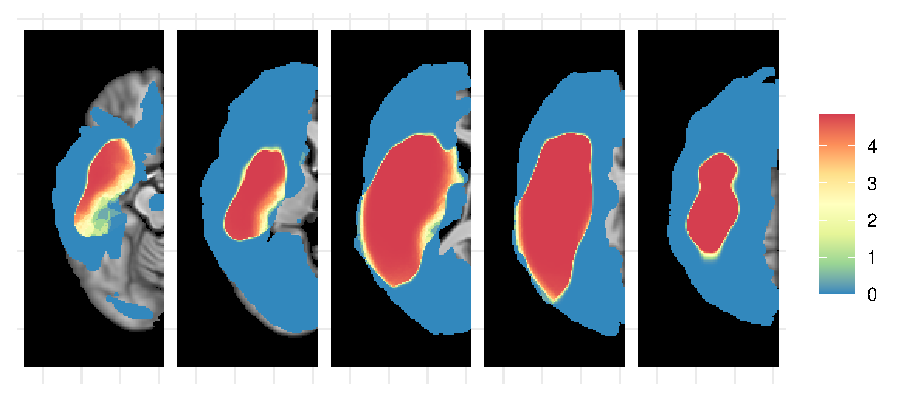
\includegraphics[trim= 2cm 0cm 1.5cm 0cm, clip, scale=0.6]{Figures/weight_wabh.pdf} &
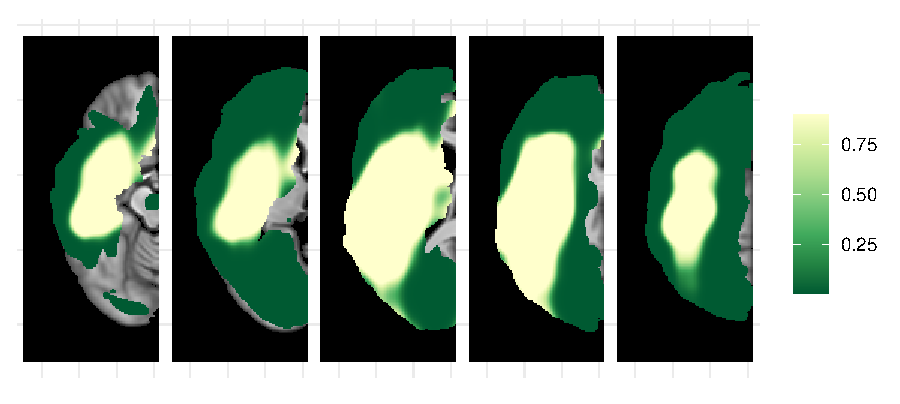
\includegraphics[trim= 2cm 0cm 1.5cm 0cm, clip, scale=0.6]{Figures/pihat_camt.pdf} \\
(c) & (d) \\
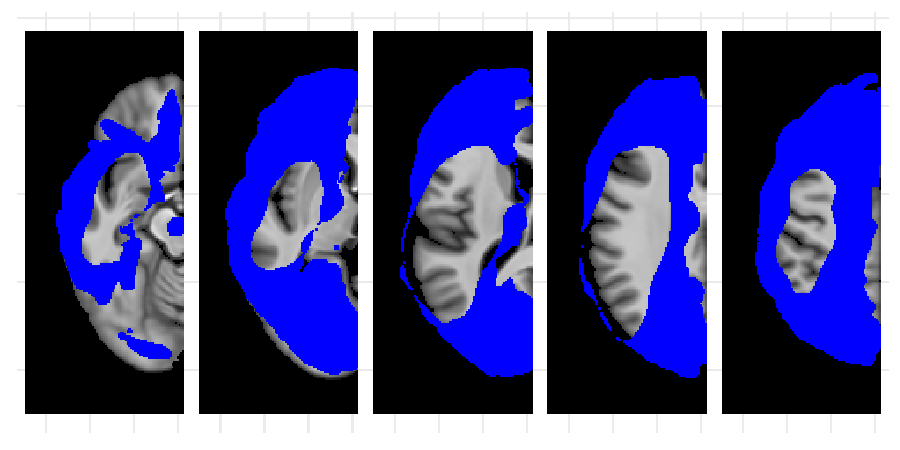
\includegraphics[trim= 3cm 0cm 3cm 0cm, clip, scale=0.72]{Figures/incon_wabh.pdf}&
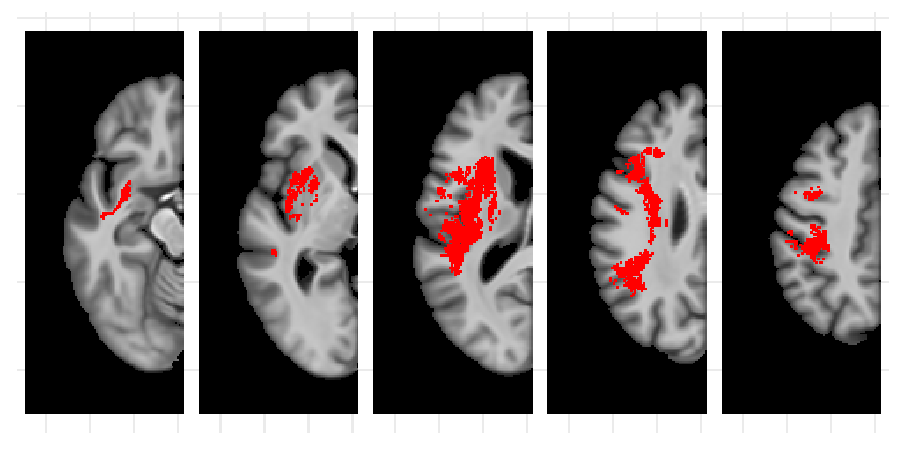
\includegraphics[trim= 3cm 0cm 3cm 0cm, clip, scale=0.72]{Figures/dis_wabh.pdf} \\
\end{tabular}
\caption{For the WABH procedure with CAMT estimated $\pi_m$ with $\tau = \max(\pi_m)$ (a) p-value weights, (b) estimated $\pi_m$, (c) inconclusive voxels (blue), and (c) significant voxels (red) for the WABH procedure.  The plots are overlayed on a structural brain image for reference.}\label{fig.data.weights}
\end{figure}

Lesion status was regressed as a function of the Aphasia Quotient (AQ) score ($Y$) and total lesion size \citep[$X^+$, which is commonly used in VLSM analyses,][]{Roretal07}.  Checking the assumptions of all tests individually is not possible, so scatterplots of $Y$ and $X^+$ were examined to determine the nature of the relationship between $Y$ and $X_{m}$.  This should suffice since $X^+$ is a measure of the average probability, and if the average probability is related to some transformation of $Y$ then it is plausible that the voxel-level probabilities are related to the same transformation. Scatterplots of $Y$ and $X^+$ showed a linear relationship when both were logit transformed. As a result, both $Y$ and $X^+$ were included in the model after a logit transformation.



In Figure \ref{fig.data.weights}, we present a map of the estimated p-value weights, inconclusive voxels, and significant voxels for the WABH procedure with prior non-null probability estimated using CAMT.  By knowing the weights, voxels where the tests were inconclusive can be shown. For example, the blue voxels in Figure \ref{fig.data.weights} have weights less than $0.1$ and thus could likely contain type II errors. Such results are critical to show researchers which areas still require further study. Other weight metrics show that the WABH with AdaPT resulted in 36\% up-weighted tests, 64\% inconclusive tests, and $2.79$ as the maximum weight. The WABH procedure with CAMT has 23\% up-weighted tests, 75\% inconclusive tests, and $4.84$ as the maximum weight. 

The WABH with CAMT, AdaPT, and CAMT find $26568$, $20$, and $174953$ significant voxels, respectively, while WABH with AdaPT, 10\% Rule, BH, and ABH find no significant voxels. Many of the significant voxels for WABH with CAMT appear to be located in and around the inferior frontal gyrus, which contains Broca's region, which is a main area linked to speech production.


\section{Discussion}\label{sec.disc}


In this paper, we proposed the use of weighted adaptive BH hypothesis testing for VLSM analysis. While the weighted adaptive BH procedure has been proposed by others, this paper was the first to incorporate heterogeneous prior non-null probability and proposed approach for estimating effect sizes in a manner consistent with anticipated low power assumptions of VLSM (see Theorem 3.1). The specific weighting scheme is available in Algorithm 1. Our simulation studies showed that our proposed method has a better performance than the other commonly used procedures. Specifically, we found that while CAMT has high power the $FDR$ was well above the nominal level, particularly in settings with a smaller expected effect size ($\theta$) or a number of non-nulls ($K$). LAWS also had difficulty controlling the FDR for low expected effect size. An in-depth assessment of why these methods -- both of which have solid theoretical guarantees on their FDR values -- fail to control the FDR is beyond the scope of this paper. However, it is evident that these methods have difficulty when $\theta$ and $K$ are small. As a result, their inflated FDRs are in situations where estimating properties about $\pi_m$ and $f_m$ are challenging due to low power and/or a small number of non-null tests. The proposed method was the most powerful among those that controlled the FDR for most settings. The findings of the data analysis are consistent with the findings of the simulation study, where CAMT (AdaPT) found many more (less) significant voxels than our proposed method.

While the simulation studies demonstrated sound FDR control for the proposed method in various settings, theoretical FDR control cannot be guaranteed since weights were estimated using the test data. Theoretical FDR control using the WABH procedure would require estimating weights using independent data via sample splitting or data from a similar study. A challenge with sample splitting in VLSM analyses is the sparseness of the $X_m$ variables, as estimating weights for test $m$ requires $X_{im}=1$ for some $i$. In our data analysis, among candidate voxels $360038$ (43.1\%) had damage in less than $11$ ($5\%$) subjects. Thus, a test sample of 20\% of the data ($44$ subjects) could result in $10^5$ voxels with $X_{im}=0$ for all $i$ (unestimable weights), with many others being based on a few non-zero $X$. Additionally, our simulation studies suggest that the anticipated power loss incurred from data splitting was not warranted in the settings of interest, given that FDR control was provided or very nearly provided in all simulation settings. This issue led us to exclude sample splitting in the data analysis; however, developing methods that use data-driven weights with theoretical FDR control is an area of future study. Our proposed WABH procedure ignored the dependence between the hypotheses tests. The WABH procedure has been shown to provide asymptotic FDR control under a weak dependence structure on the p-values \citep{Habiger2017}, which is plausible for our setting. However, extending the WABH to more general dependence scenarios is of interest.


In the data analysis, the number of discoveries was positively associated with the severity of weighting (i.e., heavier weighting resulted in more discoveries). However, heavy weighting results in many inconclusive hypotheses (up to 75\% in our data analysis), and the regions are likely to include type II errors which need to be studied further. P-value weighting results in more discovered voxels by down-weighting voxels where discovery isn't likely and up-weighting voxels where it is. The result is more overall power in exchange for essentially not testing some voxels. It is important to acknowledge these later regions in reporting. This is why results such as Figure \ref{fig.data.weights} should be included when they are employed so that the impact of weighting is transparent. The codes and data to replicate the data analyses are available on GitHub \cite{McLZhe22}.


\section*{Acknowledgements}
The authors gratefully acknowledge that this research has been supported by the National Institutes of Health grant (R01 DC009571) to CR and JF.

\bibliographystyle{asa}
\bibliography{WeightedMultipleTesting}

\end{document}